\newcommand{\nom}{Porte conteneur}
\newcommand{\sequence}{03}
\newcommand{\num}{04}
\newcommand{\type}{TD}
\newcommand{\descrip}{Résolution d'un problème en utilisant des méthodes algorithmiques}
\newcommand{\competences}{Alt-C3: Concevoir un algorithme répondant à un problème précisément posé}
\documentclass[10pt,a4paper]{article}
  \usepackage[french]{babel}
  \usepackage[utf8]{inputenc}
  \usepackage[T1]{fontenc}
  \usepackage{xcolor}
  \usepackage[]{graphicx}
  \usepackage{makeidx}
  \usepackage{textcomp}
  \usepackage{amsmath}
  \usepackage{amssymb}
  \usepackage{stmaryrd}
  \usepackage{fancyhdr}
  \usepackage{lettrine}
  \usepackage{calc}
  \usepackage{boxedminipage}
  \usepackage[french,onelanguage, boxruled,linesnumbered]{algorithm2e}
  \usepackage[colorlinks=false,pdftex]{hyperref}
  \usepackage{minted}
  \usepackage{url}
  \usepackage[locale=FR]{siunitx}
  \usepackage{multicol}
  \usepackage{tikz}
  \makeindex

  %\graphicspath{{../Images/}}

%  \renewcommand\listingscaption{Programme}

  %\renewcommand{\thechapter}{\Alph{chapter}}
  \renewcommand{\thesection}{\Roman{section}}
  %\newcommand{\inter}{\vspace{0.5cm}%
  %\noindent }
  %\newcommand{\unite}{\ \textrm}
  \newcommand{\ud}{\mathrm{d}}
  \newcommand{\vect}{\overrightarrow}
  %\newcommand{\ch}{\mathrm{ch}} % cosinus hyperbolique
  %\newcommand{\sh}{\mathrm{sh}} % sinus hyperbolique

  \textwidth 160mm
  \textheight 250mm
  \hoffset=-1.70cm
  \voffset=-1.5cm
  \parindent=0cm

  \pagestyle{fancy}
  \fancyhead[L]{\bfseries {\large PTSI -- Dorian}}
  \fancyhead[C]{\bfseries{{\type} \no \numero}}
  \fancyhead[R]{\bfseries{\large Informatique}}
  \fancyfoot[C]{\thepage}
  \fancyfoot[L]{\footnotesize R. Costadoat, C. Darreye}
  \fancyfoot[R]{\small \today}
  
  \definecolor{bg}{rgb}{0.9,0.9,0.9}
  
  
  % macro Juliette
  
\usepackage{comment}   
\usepackage{amsthm}  
\theoremstyle{definition}
\newtheorem{exercice}{Exercice}
\newtheorem*{rappel}{Rappel}
\newtheorem*{remark}{Remarque}
\newtheorem*{defn}{Définition}
\newtheorem*{ppe}{Propriété}
\newtheorem{solution}{Solution}

\newcounter{num_quest} \setcounter{num_quest}{0}
\newcounter{num_rep} \setcounter{num_rep}{0}
\newcounter{num_cor} \setcounter{num_cor}{0}

\newcommand{\question}[1]{\refstepcounter{num_quest}\par
~\ \\ \parbox[t][][t]{0.15\linewidth}{\textbf{Question \arabic{num_quest}}}\parbox[t][][t]{0.85\linewidth}{#1\label{q\the\value{num_quest}}}\par
~\ \\}

\newcommand{\reponse}[4][1]
{\noindent
\rule{\linewidth}{.5pt}\\
\textbf{Question\ifthenelse{#1>1}{s}{} \multido{}{#1}{%
\refstepcounter{num_rep}\ref{q\the\value{num_rep}} }:} ~\ \\
\ifdef{\public}{#3 ~\ \\ \feuilleDR{#2}}{#4}
}

\newcommand{\cor}
{\refstepcounter{num_cor}
\noindent
\rule{\linewidth}{.5pt}
\textbf{Question \arabic{num_cor}:} \\
}

%%\usepackage[a4paper]{geometry}
%\geometry{margin={1cm,1.2cm}}
%\usepackage[francais]{babel}
%\usepackage{nopageno} %pas de numérotation de page
%\pagestyle{plain} %numérotation en bas de page, pas d'entête
%\usepackage{hyperref}
%\usepackage[latin1]{inputenc}

%%%%%%%%%%%%%%%%%%%%%%%%%%%%%%%%%%%%%%%%%%%%%%%%%%%%%%%%%%%%%%%%%%%%%%%%%%%%%%%%%%%%%

\usepackage{amsthm}
\usepackage{amscd}
%\usepackage{mathrsfs}
%\usepackage{amsfonts}
%\usepackage[T1]{fontenc}
%\usepackage{theorem}
\usepackage{lscape}
\usepackage{variations}  % pour faire des tableaux de variations
\usepackage{dsfont}
\usepackage{fancyvrb} % pour mettre Verbatim dans une box

% Pour les figures
\usepackage{subfig}
%\usepackage{calc} % Pour pouvoir donner des formules dans les d�finitions de longueur
%\usepackage{graphicx} % Pour inclure des graphiques 
% Attention : pour inclure des .jpg comme dans l'exemple (ou des .png ou .pdf)
% il faut compiler directement en pdf (commande pdflatex).
% Pour inclure des .eps, il faut compiler avec latex + dvips + ps2pdf.
\usepackage{psfrag}
%\usepackage{color}

%%%%%%%%%%%%%%%%%%%%%%%%%%%%%%%%%%%%%%%%%%%%%%%%%%%%%%%%%%%%%%%%%%%%%%%%%%%%%%%%%%%%%

\theoremstyle{definition}
\newtheorem*{thm}{Théorème}
%\theorembodyfont{\rmfamily}
\newtheorem*{defn}{Définition}
\newtheorem{exercice}{Exercice}
\newtheorem*{problem}{Problème}
\newtheorem*{prop}{Proposition}
\newtheorem*{corollaire}{Corollaire}
\newtheorem*{lemme}{Lemme}
\newtheorem*{remark}{Remarque}
\newtheorem*{notation}{Notation}
\newtheorem*{ex}{Exemple}
\newtheorem*{ppe}{Propriété}
\newtheorem*{meth}{Méthode}
\newtheorem*{rappel}{Rappel}
\newtheorem*{voca}{Vocabulaire}
\setlength{\columnseprule}{0.5pt}


%%%%%%%%%%%%%%%%%%%%%%%%%%%%%%%%%%%%%%%%%%%%%%%%%%%%%%%%%%%%%%%%%%%%%%%%%%%%%%%%%%%%%

\newcommand{\bi}{\bigskip}
\newcommand{\dsp}{\displaystyle}
\newcommand{\noi}{\noindent}
\newcommand{\ov}{\overline}
\newcommand{\dsum}{\displaystyle \sum}
\newcommand{\dprod}{\displaystyle \prod}
\newcommand{\dint}{\displaystyle \int}
\newcommand{\dlim}{\displaystyle \lim}

%%%%%%%%%%%%%%%%%%%%%%%%%%%%%%%%%%%%%%%%%%%%%%%%%%%%%%%%%%%%%%%%%%%%%%%%%%%%%%%%%%%%%


%\newcommand{\pgcd}{\mathrm{pgcd}} % pgcd
%\providecommand{\norm}[1]{\lVert#1\rVert} % norme
%\DeclareMathOperator{\Tan}{Tan}  % espace tangent


\newcommand{\N}{\mathbb{N}}
\newcommand{\Z}{\mathbb{Z}}
\newcommand{\Q}{\mathbb{Q}}
\newcommand{\R}{\mathbb{R}}
\newcommand{\C}{\mathbb{C}}
\newcommand{\K}{\mathbb{K}}
\newcommand{\U}{\mathbb{U}}
\newcommand{\Tr}{\text{Tr}\,}
\newcommand{\pg}{\geqslant}
\newcommand{\pp}{\leqslant}
\newcommand{\bul}{\item[$\bullet$]}
\newcommand{\card}{\text{Card}}
\newcommand{\re}{\text{Re}\;}
\newcommand{\im}{\text{Im}\;}
\newcommand{\Ker}{\text{Ker}\;}
\newcommand{\Vect}{\text{Vect}\;}
\newcommand{\rg}{\text{rg}\;}
\newcommand{\TT}{{}^t\!}
%\newcommand{\sh}{\text{sh}}
%\newcommand{\ch}{\text{ch}}
\newcommand{\Mat}{\text{Mat}}
\usepackage{textcomp}



%%%%%%%%%%%%%%%%%%%%%%%%%%%%%%%%%%%%%%%%%%%%%%%%%%%%%%%%%%%%%%%%%%%%%%%%%%%%%%%%%%%%%%%%%%%%%%%%%%%%%%%%%%%%%%%%%%%%%%%%%%%





\ifdef{\public}{\excludecomment{solution}}

\begin{document}

\begin{center}
{\Large\bf TP \no {\numero} -- \descrip}
\end{center}


\SetKw{KwFrom}{de} 

\section{Recherche d'un élément dans un tableau trié}

La donnée est un tableau $L$ de valeurs réelles \textbf{triées}. L'objectif est de trouver une valeur $a$ dans ce tableau.

\subsection{Première approche naïve}

La première méthode est de parcourir le tableau terme à terme, en commençant par $L[0]$ jusqu'à tomber sur $a$.

\begin{exercice}
Ecrire une fonction \verb?recherche_naive? qui prend comme entrée \verb?L? et \verb?a? et renvoie la position de \verb?a? si $a$ est dans le tableau et \verb?False? sinon.
\end{exercice}

\begin{solution}~\\
\vspace{-0.7cm}
\begin{minted}{python}
def recherche_naive(L,a):
    i=0
    while L[i]<a:
		i=i+1
	if l[i]==a:
		return(i)
	else:
		return(False)    	
\end{minted}    
\end{solution}


\begin{exercice}
Combien d'étapes sont nécessaires dans l'algorithme précédent ?
\end{exercice}

\begin{solution}
On a fait autant d'étapes que la position renvoyée.
\end{solution}




\subsection{R\' esolution par dichotomie}

L'algorithme dichotomique permet une recherche de $a$ plus rapide. Le principe en est le suivant :\\
$m$ est l'indice du milieu du tableau $L$.
\begin{itemize}
\item si $L[m]$ vaut $a$, on renvoie $m$ ;
\item si $L[m]>a$, on recommence dans la moitié supérieure du tableau ;
\item si $L[m]<a$, on recommence dans la moitié inférieure.
\end{itemize}


\begin{exercice}A la main.
\begin{enumerate}
\item Dans le tableau de taille 15 suivant : $L=[-1,0,1,3,4,5,6,8,9,10,12,13,14,15,16]$, déterminer les étapes successives pour trouver la position de $a=12$, par une recherche dichotomique.
\item Faites de même avec $L=[-2,-1,0,2,3,4,8,9]$ et $a=8$.
\end{enumerate}
\end{exercice}

\begin{solution}
On travaille à chaque fois sur des sous-tableaux de $L$. On notera $d$ l'indice le plus petit du sous-tableaux et $f$ le plus grand. A chaque étape, voici les valeurs les sous tableaux sur lesquels on travaille :
\begin{enumerate}
\item $L$, $d=0,f=14,m=7,L[m]=8$.
\item $[9,10,12,13,14,15,16]$, $d=9,f=14,m=11,L[m]=13$.
\item $[9,10,12]$, $d=8,f=10,m=9,L[m]=10$.
\item $[12]$, $d=10,f=10,m=10,L[m]=12$.
\end{enumerate}
Pour la deuxième liste : 
\begin{enumerate}
\item $L$ $d=0,f=8,m=3,L[m]=2$.
\item $[3,4,8,9]$, $d=4,f=8,m=5,L[m]=4$.
\item $[8,9]$, $d=6,f=8,m=6,L[m]=8$.
\end{enumerate}
\end{solution}


\begin{exercice}
En reprenant le principe de la dichotomie, écrire une fonction \verb?dicho? qui prend comme entrée \verb?L? et \verb?a? et renvoie la position de \verb?a? si $a$ est dans le tableau et \verb?False? sinon.
\end{exercice}

\begin{solution}~\\
\vspace{-0.7cm}
\begin{minted}{python}
def dichotomie(L, a):
    debut = 0
    fin = len(L) - 1
    while debut <= fin:
        m = (debut+fin) // 2
        if L[m] == a:
            return m
        elif L[m] < a:
            debut = m + 1
        else:
            fin = m - 1
    return False
\end{minted}
\end{solution}

\begin{remark}
Essayez sans, mais si vous avez des difficultés, reportez-vous au pseudo code en annexe.
\end{remark}


\begin{exercice}
Vérifier que votre fonction est correcte : si $i$ est l'indice renvoyé par \verb?dicho?, que doit retourner \verb?L[i]? ?
\end{exercice}

\begin{solution}
\verb?L[dicho(L,a)]=a?
\end{solution}



\begin{exercice}Comparaison recherche naïve/dichotomie.\\
Modifier votre focntion \verb?dicho? en une fonction \verb?dicho_comparatif? qui prend comme entrée \verb?L? et \verb?a? et renvoie le nombre d'étapes qu'il a été nécessaire pour trouver la position de \verb?a?. \\
Comparer sur des mêmes exemples le nombre d'étapes nécessaires pour la recherche naïve et pour la dichotomie.
\end{exercice}

\begin{solution}~\\
\vspace{-0.7cm}
\begin{minted}{python}
def dichotomie_comparatif(L, a):
    debut = 0
    fin = len(L) - 1
    compteur=0
    while debut <= fin:
        compteur=compteur+1
        m = (debut+fin) // 2
        if L[m] == a:
            return m,compteur
        elif L[m] < a:
            debut = m + 1
        else:
            fin = m - 1
    return False,compteur
\end{minted}
\end{solution}



\begin{remark}Complexité des deux algorithmes.\\
La complexité d'un algorithme donne une idée du nombres d'étapes nécessaires pour qu'un algorithme se termine.\\
Dans le cas de la recherche naïve, dans le pire des cas, on fera $n$ étapes (si l'élément est en dernier). On dit que la complexité est linéaire, qu'elle est en $O(n)$.\\
Dans le cas de la recherche par dichotomie, on peut montrer que la complexité est en $O(\log(n))$ : elle est beaucoup plus rapide.
\end{remark}



\section{Recherche du zéro d'une fonction}

Dans cette section, le tableau $L$ contient des valeurs réelles qui représentent les valeurs prises par une fonction croissante. On cherche à trouver quand est-ce que la fonction s'annule.

\begin{exercice}
En utilisant le principe de la recherche par dichotomie, écrire une fonction \verb?dicho_zero? qui prend comme entrée un tableau à valeurs triées $L$ et qui renvoie l'indice $i$ tel que $L[i]$ est la valeur la plus proche de zéro dans le tableau $L$.
\end{exercice}

\begin{solution}~\\
\vspace{-0.7cm}
\begin{minted}{python}
def dicho_zero(L):
    debut = 0
    fin = len(L) - 1
    while debut <= fin:
        m = (debut+fin) // 2
        if L[m] == 0:
            return m
        elif L[m] < 0:
            debut = m + 1
        else:
            fin = m - 1
    return(m)
\end{minted}    
\end{solution}

\begin{exercice}
Testez la fonction précédente sur $L=[-2,-1,2,3]$. Proposer une fa\c con de vérifier le résultat.
\end{exercice}

\begin{solution}
Si \verb?dicho(L)? renvoie \verb?i?, on peut afficher \verb?L[i-1],L[i],L[i+1]?.
\end{solution}

\begin{exercice}
On considère la fonction suivante : $f(x)=x+\exp(x)$ (qui est croissante).
\begin{enumerate}
\item Construire un tableau $X$ qui contient 1000 réels équirépartis entre -1 et 1.
\item Construire un tableau $L$ qui contient les valeurs de $f$ pour chaque $x\in X$.
\item \label{zero} Avec la fonction \verb?dicho_zero?, déterminer une valeur approchée de $x$ tel que $f(x)=0$.
\item A l'aide de la notice du concours ci-dessous, tracez le graphe de la fonction $f$.
\item Vérifiez graphiquement le résultat trouvé à la question \ref{zero}.
\end{enumerate}
\end{exercice}

\begin{solution}
\begin{enumerate}
\item ~\\ 
\vspace{-0.7cm}
\begin{minted}{python}
X=[]
x=-1
for i in range(1000):
    x=x+2/1000.
    X.append(x)
\end{minted}    
\item ~\\ 
\vspace{-0.7cm}
\begin{minted}{python}
def f(x):
    return(exp(x)+x)

L=[]
for x in X:
    L.append(f(x)) 
\end{minted}    
\item \verb?X[dicho_zero(L)]?.
\item ~\\ 
\vspace{-0.7cm}
\begin{minted}{python}
import matplotlib.pyplot as plt    
plt.plot(X,Y)  
plt.plot(X,[0]*len(X)) 
plt.show() 
\end{minted}   
\item 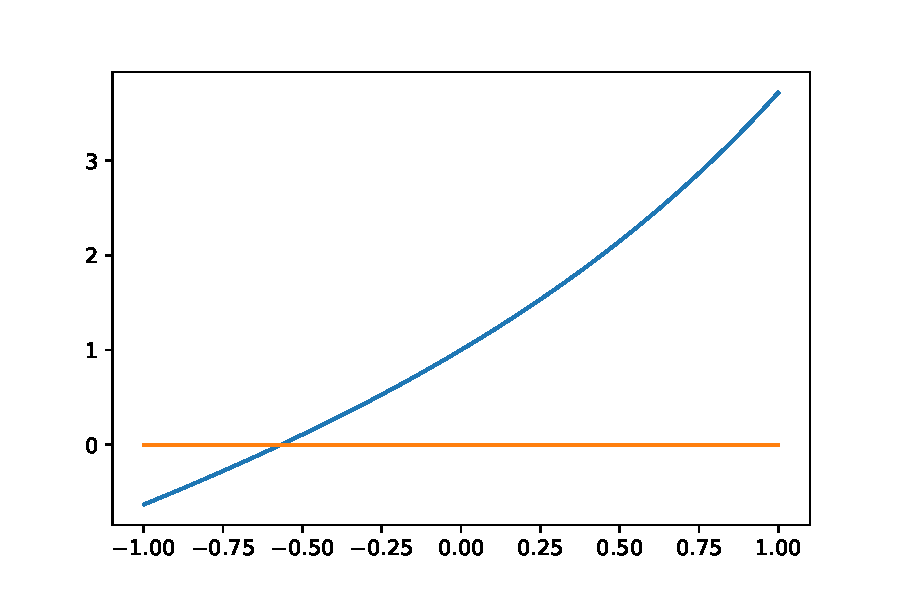
\includegraphics[scale=1]{graphe_f.pdf}
\end{enumerate}
\end{solution}

\begin{figure}[h]
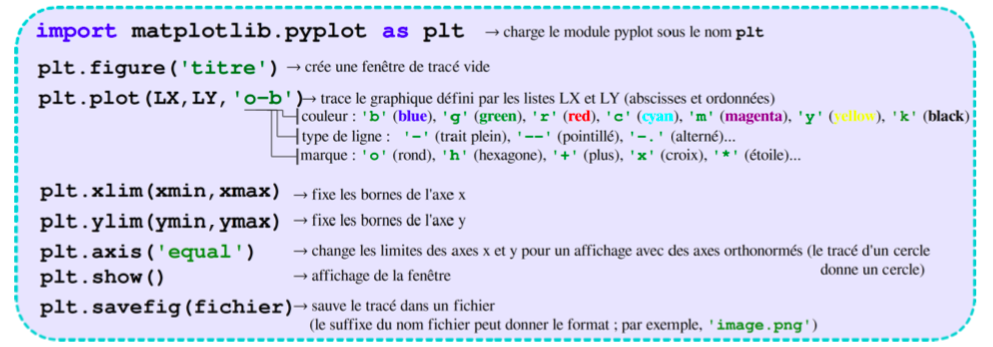
\includegraphics[scale=0.5]{memento_plt}
\caption{Documentation sur le tracé de fonctions}
\end{figure}



\section{Annexe}


\begin{algorithm}[H]
\KwData{L une liste triée de $n$ éléments et $a$ un élément}
debut $\leftarrow $premier indice de $L$ \;
fin $\leftarrow $dernier indice de $L$ \;
\textbf{Tant que} debut inférieur ou égal à fin \\
\qquad $m \leftarrow $ quotient de fin+debut par $2$\\
\qquad \textbf{si} $L[m] == a$\\
\qquad \qquad \textbf{retourner} m\\
\qquad \textbf{ou si} $L[m]<a$\\
\qquad \qquad debut$\leftarrow $m+1\\
\qquad \textbf{sinon}\\
\qquad \qquad fin$\leftarrow $m-1\\
\textbf{retourner} False
\caption{Recherche par dichotomie.}
\end{algorithm}



\end{document}








\end{document}


















